\section{Auswertung}
\label{sec:Auswertung}
\subsection{Bestimmung der Zeitkonstante anhand der Aufladekurve}
Um die Aufladekurve des RC-Gliedes zu erhalten, wird der in der Durchführung beschriebene Aufbau betrachtet.
Es ergibt sich das in Abbildung \ref{fig:oz1} dargestellte Bild am Oszillographen, welches die Aufladekurve des betrachteten RC-Gliedes darstellt.

\begin{figure}[H]
  \centering
  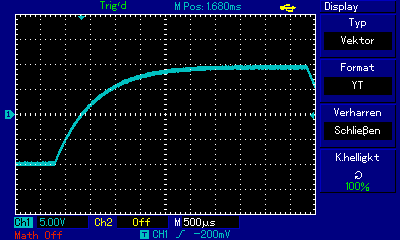
\includegraphics{oz4.png}
  \caption{Aufladekurve des RC-Gliedes.}
  \label{fig:oz1}
\end{figure}

Hierbei ist auf der x-Achse die Zeit $t$ in $\SI{500}{\micro\second}$ pro Kästchen, auf der y-Achse die Kondensatorspannung $U_c$ in $\SI{5}{\volt}$ pro Kästchen aufgetragen.
Um nun eine lineare Ausgleichsrechnung zur Bestimmung der Zeitkonstante $\tau$ durchführen zu können, werden dem Graphen die in Tabelle \ref{tab:werte_a} angegebenen Werte entnommen.


\begin{table}[H]
  \centering
  \caption{Messwerte der Aufladekurve des Kondensators.}
  \label{tab:werte_a}
  \sisetup{table-format=1.2}
  \begin{tabular}{c c}
    \toprule
    {$U_c [\si{\milli\second}]$} & {$t [\si{\volt}]$}\\
    \midrule
    \input{build/atabelle.tex}
    \bottomrule
  \end{tabular}
\end{table}

Da sich die Werte wie in \eqref{eqn:gl2} angegeben verhalten, kann nicht direkt eine lineare Ausgleichsrechnung durchgeführt werden.
Zuerst müssen die Werte in die Form
\begin{equation}
  U_c' = U_0 \mathrm{e}^{\frac{-t}{RC}}
\end{equation}
gebracht werden.
Dazu wird von den $U_c$ Werten der Wert $U_{\text{end}} = \SI{19.5}{\volt}$ abgezogen sowie das Vorzeichen umgekehrt.
Es ergeben sich hieraus die in Tabelle \ref{tab:werte_a_neu} angegebenen Werte, so dass die Werte $t$ und $\log(U_c')$ an die Funktion
\begin{equation}
  y = m x +b
\end{equation}
gefittet werden können.

\begin{table}[H]
  \centering
  \caption{Veränderte Messwerte der Aufladekurve.}
  \label{tab:werte_a_neu}
  \sisetup{table-format=1.2}
  \begin{tabular}{c c}
    \toprule
    {$U_c [\si{\milli\second}]$} & {$t [\si{\volt}]$}\\
    \midrule
    \input{build/atabelle_neu.tex}
    \bottomrule
  \end{tabular}
\end{table}

Die Ausgleichsrechnung wird durch die Methode der kleinsten Quadrate mit numpy in Python durchgeführt.
Das Ergebnis ist die in Abbildung \ref{fig:plot_a} halblogarithmisch dargestellte Ausgleichsgerade.
Die sich ergebenen Parameter des Fits sind
\begin{align*}
  m &= \input{build/fit_3_m.tex}, \\
  b &= \input{build/fit_3_b.tex}.
\end{align*}
Mit
\begin{equation}
  RC = \frac{-1}{m}
\end{equation}
ergibt sich der zu bestimmende RC-Wert zu
\begin{align}
  RC &= \input{build/wert_rc_a.tex}.
\end{align}
\begin{figure}[H]
  \centering
  \includegraphics{aplot.pdf}
  \caption{Ausgleichsgerade zur Bestimmung von RC.}
  \label{fig:plot_a}
\end{figure}

\subsection{Methode der Kondensatoramplitude und Phasenverschiebung}
Abgesehen vom Betrachten der Aufladekurve, kann die Zeitkonstante $RC$ auch durch die Amplitude der Kondensatorspannung $U_C$ und die Phasenverschiebung $\phi$ der beiden Spannungen berechnet werden.
In Tabelle \ref{tab:2} sind die nötigen Messdaten aufgelistet.
%
%\begin{table}
%  \centering
%  \caption{Messdaten zur Frequenzabhängigen Amplituden und Phasenverschiebungsbestimmung.}
%  \label{tab:2}
%  \sisetup{table-format=5.2}
%  \begin{tabular}{c c c c}
%    \toprule
%    {$f [\si{\hertz}]$} & {$U_C [\si{\milli\volt}]$} & {$a [\si{\micro\second}]$} & {$b [\si{\micro\second}]$}\\
%    \midrule
%    \input{build/bctabelle.tex}
%    \bottomrule
%  \end{tabular}
%\end{table}
%

\begin{table}
  \hspace*{\fill}
  \begin{subfigure}{0.40\textwidth}
  \centering
  %\caption{Messdaten Teil 1.}
  \label{tab:2a}
  \sisetup{table-format=3.4}
  \begin{tabular}{c c c c}
    \toprule
     {$f [\si{\hertz}]$} & {$U_C [\si{\milli\volt}]$} & {$a [\si{\micro\second}]$} & {$b [\si{\micro\second}]$}\\
    \midrule
    \input{build/frequenztabelle1.tex}
    \bottomrule
  \end{tabular}
\end{subfigure}
\hspace*{\fill}
\begin{subfigure}{0.40\textwidth}
  \centering
  %\caption{Messdaten Teil 2.}
  \label{tab:2b}
  \sisetup{table-format=3.4}
  \begin{tabular}{c c c c}
    \toprule
    {$f [\si{\hertz}]$} & {$U_C [\si{\milli\volt}]$} & {$a [\si{\micro\second}]$} & {$b [\si{\micro\second}]$}\\
    \midrule
    \input{build/frequenztabelle2.tex}
    \bottomrule
  \end{tabular}
\end{subfigure}
\\
\hspace*{\fill}
\hspace*{\fill}
\caption{Messdaten zur Frequenzabhängigen Amplituden und Phasenverschiebungsbestimmung.}
\label{tab:2}
\end{table}
%\begin{table}
%  \centering
%  \caption{Messdaten zur Frequenzabhängigen Amplituden und Phasenverschiebungsbestimmung.}
%  \label{tab:2}
%  \sisetup{table-format=5.2}
%  \begin{tabular}{c c c c c c c c}
%    \toprule
%    {$f [\si{\hertz}]$} & {$U_C [\si{\milli\volt}]$} & {$a [\si{\micro\second}]$} & {$b [\si{\micro\second}]$} & {$f [\si{\hertz}]$} & {$U_C [\si{\milli\volt}]$} & {$a [\si{\micro\second}]$} & {$b [\si{\micro\second}]$}\\
%    \midrule
%    \input{build/frequenztabelle.tex}
%    \bottomrule
%  \end{tabular}
%\end{table}


%
%\begin{table}
%  \centering
%  \caption{Messdaten zur Frequenzabhängigen Amplituden und Phasenverschiebungsbestimmung.}
%  \label{tab:8}
%  \sisetup{parse-numbers=false}
%  \begin{tabular}{
%    S[table-format=1.3]
%    S[table-format=1.3]
%    @{${}{}{}{}$}
%    %S[table-format=1.2]
%    @{\hspace*{3em}\hspace*{\tabcolsep}}
%    S[table-format=1.3]
%    S[table-format=1.3]
%    @{${}{}{}{}$}
%    %S[table-format=1.2]
%  }
%    \toprule
%    {$v \:/\: \si{\hertz}$} & {$U_{\text{Br}} \:/\: \si{\volt}$} & {$v \:/\: \si{\hertz}$} & {$U_{\text{Br}} \:/\: \si{\volt}$} &
%    {$v \:/\: \si{\hertz}$} & {$U_{\text{Br}} \:/\: \si{\volt}$} & {$v \:/\: \si{\hertz}$} & {$U_{\text{Br}} \:/\: \si{\volt}$} \\
%    \midrule
%    \input{build/frequenztabelle.tex}
%    \bottomrule
%  \end{tabular}
%\end{table}
%
Dabei bezeichnet $f$ die Erregerfrequenz, $a$ den Abstand zweier Nulldurchläufe und $b$ die Periodendauer der Erregerfrequenz.
In Abbildung \ref{abb:3} werden die gemessenen mit der Erregerspannung normierten Amplituden gegen die Kreisfrequenz der Erregerspannung halblogarithmisch eingetragen.

\begin{figure}[H]
  \centering
  \includegraphics{bplot.pdf}
  \caption{Normierte Kondensatoramplituden.}
  \label{abb:3}
\end{figure}

Mittels eines Fits der Form
\begin{equation}
  f = \frac{1}{\sqrt{1+x²m²}} +b,
\end{equation}
werden die Messwerte gefittet.
Die Parameter werden dabei zu
\begin{align*}
  m &= \input{build/fit_1_m.tex}, \\
  b &= \input{build/fit_1_b.tex},
\end{align*}
bestimmt.
Somit ergibt sich nach der Formel \eqref{fuck1} die Zeitkonstante $RC$ zu
\begin{equation}
  RC = \input{build/wert_rc_b.tex}.
\end{equation}
Die Phasenverschiebung $\phi$ kann über die Formel
\begin{equation}
  \phi = \frac{a}{b} \cdot 2\pi
\end{equation}
bestimmt werden.
Diese wird ebenfalls halblogarithmisch gegen die Erregerkreisfrequenz aufgetragen.
Dies realisiert Abbildung \ref{abb:4}.

\begin{figure}[H]
  \centering
  \includegraphics{cplot.pdf}
  \caption{Phasenverschiebungen.}
  \label{abb:4}
\end{figure}

An dieser Stelle wird eine Funktion der Art
\begin{equation}
  f = A\arctan(mx)+b,
\end{equation}
identisch (\ref{eqn:4}), gefittet.
Die Parameter ergeben sich hier zu
\begin{align*}
  a &= \input{build/fit_2_a.tex}, \\
  m &= \input{build/fit_2_m.tex},  \\
  b &= \input{build/fit_2_b.tex}.
\end{align*}
Die nicht-lineare Ausgleichsrechnung lässt somit auf den Wert
\begin{equation}
  RC = \input{build/wert_rc_c.tex}
\end{equation}
schließen.\\
Mit letzterem Wert kann ein Polarplot erstellt werden.
Der Winkel $\phi$ beschreibt die Phasenverschiebung, der Radius hingegen die normierte Amplitude der Kondensatorspannung.
Die Phasenverschiebung wird nach Formel (\ref{fuck2}) berechnet und die normierte Amplitude ergibt sich aus Gleichung (\ref{fuck1}).
Es resultiert der Polarplot in Abbildung \ref{abb:5} mit $RC = \input{build/wert_rc_c.tex}$.

\begin{figure}[H]
  \centering
  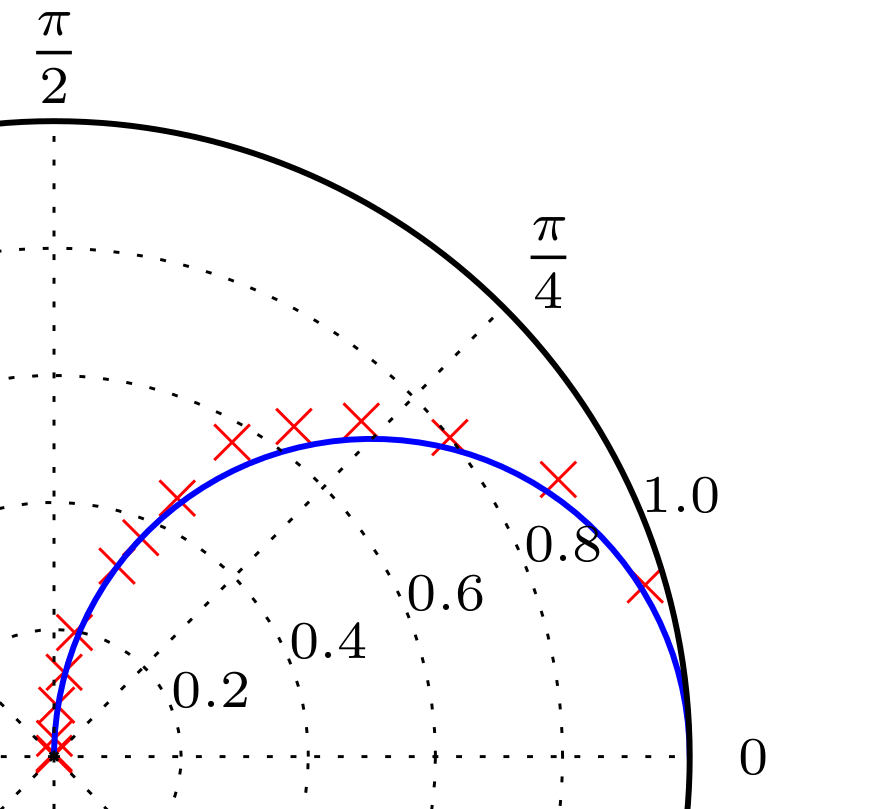
\includegraphics[height=7cm]{fake_plot.png}
  \caption{Polarplot.}
  \label{abb:5}
\end{figure}

Es werden mehrere Probewerte eingezeichnet.

\subsection{Nutzung des RC-Gliedes zur Integration}
Das RC-Glied wird, wie in der Durchführung beschrieben, zur Integration der angelegten Spannung genutzt.
Dabei wird eine Frequenz von $\nu = \SI{3000}{\hertz}$ verwendet.
Zunächst wird eine Sinusspannung angelegt, so dass
\begin{align}
U_G &= U_0\sin{\omega t}  & U_c &= -\frac{U_0}{\omega}\cos{\omega t}
\end{align}
als Spannungen erwartet werden, wobei $U_G$ die angelegte Spannung, $U_c$ die erwartete Kondensatorspannung und $U_0$ die Amplitude der Sinusspannung bezeichnet.
In Abbildung \ref{fig:sin_r} wird das abgelesene Ergebnis dargestellt.

\begin{figure}[H]
  \centering
  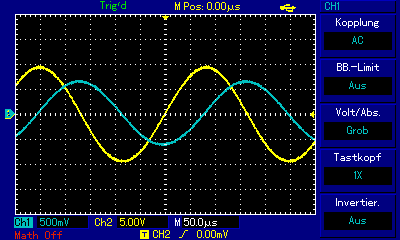
\includegraphics[height=4.5cm]{oz5.png}
  \caption{Erhaltene Kurven für Sinusspannung.}
  \label{fig:sin_r}
\end{figure}


Als nächstes wird die Rechteckspannung überprüft, so dass die Werte
\begin{align}
  U_G &=
  \begin{cases}
    U_0 , &  0 \leq t \leq \frac{T}{2} \\
    -U_0 , & \frac{T}{2} \leq t \leq T
  \end{cases}
   & U_c &=
  \begin{cases}
    at , &  0 \leq t \leq \frac{T}{2} \\
    -at , & \frac{T}{2} \leq t \leq T
  \end{cases}
\end{align}
mit $U_0$ als Amplitude der Rechteckspannung sowie $a$ als positiven Skalierungsfaktor erwartet werden.
Abbildung \ref{fig:rechteck_s} zeigt das am Oszillographen abgelesene Bild.

\begin{figure}[H]
  \centering
  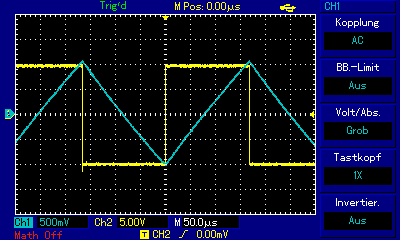
\includegraphics[height=4.5cm]{oz7.png}
  \caption{Erhaltene Kurven für Rechteckspannung.}
  \label{fig:rechteck_s}
\end{figure}

Zum Schluss wird die Dreieckspannung überprüft, woraus sich die erwarteten Werte
\begin{align}
  U_G &=
  \begin{cases}
    at , &  0 \leq t \leq \frac{T}{2} \\
    -at , & \frac{T}{2} \leq t \leq T
  \end{cases}
  & U_c &=
  \begin{cases}
    b t^2 , &  0 \leq t \leq \frac{T}{2} \\
    -b t^2 , & \frac{T}{2} \leq t \leq T
  \end{cases}
\end{align}
mit Skalierungsfaktoren $a$ und $b$ ergeben.
Abbildung \ref{fig:s_s} zeigt das abgelesene Bild.

\begin{figure}[H]
  \centering
  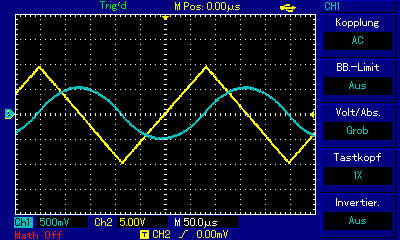
\includegraphics[height=4.5cm]{oz6.png}
  \caption{Erhaltene Kurven für Dreieckspannung.}
  \label{fig:s_s}
\end{figure}
